\documentclass{article}
\usepackage{amssymb,amsmath}
\usepackage{mathtools}
\usepackage{graphicx}
\usepackage{multicol}
\usepackage{array}
\topmargin=-0.3in
\textheight=9.2in
\textwidth=168mm
\oddsidemargin=-0.2in
\evensidemargin=-0.2in

\title{Partial Differential Equations}
\date{}
\begin{document}
\maketitle
\newpage
\section{First Order Partial Differential Equations}
\hrule
\noindent\\\\
\noindent\textbf{\textit{Ex:}} Solve the following PDE
\[
u_{x} + u_{y} + u = x + y
\]
\indent \textbf{\textit{Solution:}} In this case, we have a non-zero term on the
right hand side of the equation. We will use substitution to solve this. For the
time being, we will let $T$ be $x + y$. To find our $S$, we can use a similar
method to the one that we used above. We know that the coefficients on the
$u_{x}$ and $u_{y}$ are $1$ in this case. Now we have:
\begin{align*}
\frac{dy}{dx} &= 1\\
dy &= dx\\
\int dy &= \int dx\\
x &= y + c\\
x - y &= c
\end{align*}
\noindent Now we can say that $S = x - y$; however, we need to check our choice
for $T$ to make sure this substitution will not just yield a trivial solution.
We can do this by Next we have to actually use the substitution. We need to
determine whether the coefficient matrix, or the Jacobian, of our substitutions
has a determinant of zero. If it does, then we need to choose a different $T$.
\[
\left|
\begin{array}{c c}
1 & 1\\
1 & -1
\end{array}
\right| = 2 \neq 0.
\]
Our choices of variables will work here, so now we need to express $u_{x}$ and
$u_{y}$ in terms of $S$ and $T$. The following equations come from the chain
rule; when the $S$ and $T$ terms are differentiated, we get $u_{S}$ and $u_{T}$
left behind.
\begin{alignat*}{3}
u_{x} &= u_{S}\frac{\partial S}{\partial x} + u_{T}\frac{\partial T}{\partial x}
\qquad\qquad &&u_{y} = u_{S}\frac{\partial S}{\partial y} + u_{T}\frac{\partial T}{\partial y}\\
u_{x} &= -u_{S} + u_{T}  \qquad\qquad &&u_{y} = u_{S} + u_{T}
\end{alignat*}
\noindent We can now plug in our values into the original equation. Note that we
didn't do anything with $u$; it gets left alone. In addition, if we needed
$u_{xx}$ or $u_{yy}$, we can just differentiate again. Plugging in yields:
\begin{gather*}
(-u_{S} + u_{T}) + (u_{S} + u_{t}) + u = T\\
2u_{T} + u = T
\end{gather*}
\noindent This is just a first order ODE. Since it's not homogeneous, we need to
solve for the general solution, and then the particular solution. Let's start
with the general.
\begin{gather*}
2y^{'} + y = 0\\
2r + 1 = 0\\
r = -\frac{1}{2}\\
y = ce^{\left(-\frac{1}{2}\right)x}
\end{gather*}
\noindent In this case, we know that our $x$ is really $T$. So we finally have
$y = ce^{\left(-\frac{1}{2}\right)T}$. We will back substitute soon, but let's
find the particular solution before we do that.
\noindent Recall from ODE that we have several cases for the particular
solution. In our case, we have a linear equation on the right hand side of our
ODE. This lets us say:
\begin{gather*}
y = AT + B\\
y^{'} = A\\
\end{gather*}
\noindent Now we can substitute again into our non-homogeneous ODE as follows:
\[
2y^{'} + y = T \equiv 2A + AT + B = T
\]
\noindent And we have that $A = 1$, and $B = -2$. Now we have a final solution of:
\begin{gather*}
y = ce^{\left(-\frac{1}{2}\right)T} + T - 2\\
y = ce^{\left(-\frac{1}{2}\right)(x+y)} + (x + y) - 2
\end{gather*}
\noindent We aren't quite done yet, as we have a solution to an ODE, not a PDE.
It isn't too difficult to switch back; The $c$ is really the only difference. In
our ODE, the $c$ is a constant term, but to our PDE, the $c$ is a function. The
$c$ now becomes $f(s)$. We will go ahead and back substitute, which will give us
$f(y-x)$. Now we have our final solution:
\[
u(x,y) = f(y-x)e^{\left(-\frac{1}{2}\right)(x+y)} + (x + y) - 2
\]
\noindent And we are done.


\newpage
\section{Classification of Partial Differential Equations}
\hrule
\noindent\\\\
\indent We mentioned earlier the topic of classification of PDE's. Since we only
have this and Fourier Series to talk about, we will go ahead and knock out
classification. There's some information that we need to go ahead and review
here. This will be explained in the problem, but it's handy to have it for
reference:
\begin{align*}
b^{2} - ac < 0 &\implies \text{Elliptic with complex roots}\\
b^{2} - ac = 0 &\implies \text{Parabolic with the same root twice}\\
b^{2} - ac > 0 &\implies \text{Hyperbolic with two distinct real roots}
\end{align*}
\noindent Another helpful piece of information is what's known as the
\textit{classical trinity} of PDEs.
\begin{align*}
u_{t} - ku_{xx} &= 0 \qquad \text{The heat equation (parabolic)}\\
u_{tt} - c^{2}u_{xx} &= 0 \qquad \text{The wave equation (hyperbolic)}\\
u_{xx} + u_{yy} &= 0 \qquad \text{The Laplace equation (elliptic)}
\end{align*}
Let's go ahead and look at an example.\\\\
\indent \textbf{Ex. }Classify the following PDE:
\[yu_{xx} + u_{yy} = 0\]
\indent \textbf{\textit{Solution:}} The first thing we need to identify are the
coefficients on the $u_{xx}$, $u_{yy}$, and $u_{xy}$ or $u_{yx}$ terms. Note
that the $u_{xy}$ and $u_{yx}$ are interchangeable. We will assign these
coefficients to $a$, $b$, and $c$ corresponding to $u_{xx}$, $u_{xy}$, and
$u_{yy}$, respectively. Looking at the PDE, we can see that
\[
a = y \qquad b = 0 \qquad c = 1
\]
\noindent Now we look at $b^{2} - ac$. We are really dealing with
$b = \frac{b_{0}}{2}$. In other words, we need to divide our $b$ value by $2$.
In the case of the first problem, we are dealing with $b = 0$. Now we can
classify our PDE as follows:
\[
b^{2} - ac = 0 - y < 0 \implies \text{Elliptic}
\]
Note that we assume $y > 0$. So our PDE is elliptic. Now we need to make it look
like it's corresponding equation from the classical trinity. In this case we
have an Elliptic equation, so we want to make it look like Laplace's equation.
We need to find values for $u_{xx}$ and $u_{yy}$, and then substitute those into
the equation. This is similar to how we solved the first order PDE's; let's look
at our characteristic equation:
\begin{gather*}
am^{2} + bm + c = 0\\
ym^{2} + 1 = 0\\
m = \pm \frac{i}{\sqrt{y}}
\end{gather*}
\noindent So, now we have two solutions, and they are both imaginary as expected.
Next we need to find values for $S$ and $T$ that we can substitute into the
equation. We will do both of them at the same time here. Notice that we will
drop the $i$:
\begin{gather*}
\frac{dy}{dx} = \frac{1}{\sqrt{y}} \qquad\qquad\qquad \frac{dy}{dx} = -\frac{1}{\sqrt{y}}\\
\int\frac{dy}{dx} =\int\frac{1}{\sqrt{y}} \qquad\qquad\qquad \int\frac{dy}{dx} = -\int\frac{1}{\sqrt{y}}\\
S = \frac{2}{3}y^{\left(\frac{3}{2}\right)} - x \qquad\qquad\qquad T = \frac{2}{3}y^{\left(\frac{3}{2}\right)} + x
\end{gather*}
\noindent Now we can substitute into our equation. Unfortunately, we will need
to take the partial derivative twice in order to get the substitutions we need.
Let's start with $u_{xx}$.
\begin{align*}
u_{x} &= u_{S}\frac{\partial S}{\partial x} + u_{T}\frac{\partial T}{\partial x}\\
&= -u_{S} + u_{T}\\
u_{xx} &= \frac{\partial}{\partial x}(-u_{S} + u_{T})\\
&= u_{SS} + u_{TT}
\end{align*}
\noindent We will skip the math for finding $u_{yy}$, which would give us
\[
u_{yy} = yu_{SS} + yu_{TT}
\]
\noindent Now we plug everything in. Remember that we were under the assumption
that $y > 0$:
\begin{gather*}
y(u_{SS} + u_{TT}) + yu_{SS} + yu_{TT} = 0\\
2yu_{SS} + 2yu_{TT} = 0\\
u_{SS} + u_{TT} = 0
\end{gather*}
\noindent And we are finished.


\newpage
\section{Fourier Series and Partial Differential Equations}
\hrule
\noindent\\
\subsection{Finding Fourier Series}
\indent It's finally time to talk about Fourier Series. Before we start though,
it may be helpful to look at some common patterns amongst the Fourier Series.\\\\
\centerline{
\bgroup
\def\arraystretch{1.5}
\begin{tabular}{|c|c|c|c|}
\hline
& Cosine & Sine & Full Series \\ \hline
Interval & $[0,L]$ & $[0,L]$ & $[-L,L]$\\ \hline
Basis & $\{1,\cos{\left(\frac{n\pi x}{L}\right)}\}$ &
$\{\sin{\left(\frac{n\pi x}{L}\right)}\}$ &
$\{1,\sin{\left(\frac{n\pi x}{L}\right)},\cos{\left(\frac{n\pi x}{L}\right)}\}$\\ \hline
Series &
$\frac{b_{0}}{2} + \sum_{n=1}^{\infty}[b_{n}\cos{\left(\frac{n\pi x}{L}\right)}]$&
$\sum_{n=1}^{\infty}[a_{n}\sin{\left(\frac{n\pi x}{L}\right)}]$&
$\frac{b_{0}}{2} + \sum_{n=1}^{\infty} [a_{n}\sin{\left(\frac{n\pi x}{L}\right)} + b_{n}\cos{\left(\frac{n\pi x}{L}\right)}]$\\ \hline
\end{tabular}
\egroup
}\\\\
\noindent To solve for the coefficients, we have:
\begin{align*}
Sine:  \qquad\qquad &a_{n} = \frac{2}{L}\int_{0}^{L}f(x)\sin{\left(\frac{n\pi x}{L}\right)}dx\\
Cosine: \qquad\qquad &b_{n} = \frac{2}{L}\int_{0}^{L}f(x)\cos{\left(\frac{n\pi x}{L}\right)}dx\\
&b_{0} =  \frac{1}{L}\int_{0}^{L}f(x)dx\\
Full: \qquad\qquad &a_{n} = \frac{2}{L}\int_{-L}^{L}f(x)\sin{\left(\frac{n\pi x}{L}\right)}dx\\
&b_{n} = \frac{2}{L}\int_{-L}^{L}f(x)\cos{\left(\frac{n\pi x}{L}\right)}dx\\
&b_{0} =  \frac{1}{L}\int_{-L}^{L}f(x)dx
\end{align*}
\indent It will also help us to quickly review the concept of odd and even
functions, as they will help us to simplify the process of computing Fourier
series later. Specifically, let's look at the graphs for $\sin$ and $\cos$ on
$[-\pi,\pi]$, as well as another function that will turn out to be neither even
nor odd.
\begin{center}
\begin{tabular}{c c c}
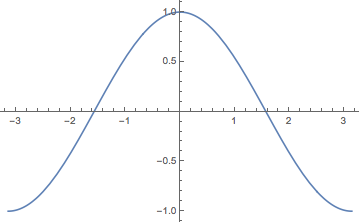
\includegraphics[scale=0.4]{cos_eo} & 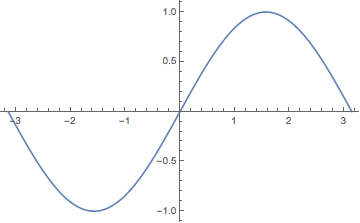
\includegraphics[scale=0.4]{sin_eo} & 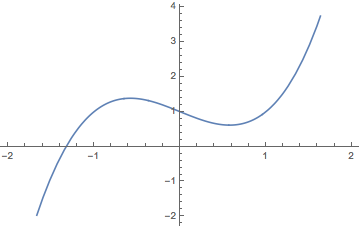
\includegraphics[scale=0.4]{cube_eo}\\
$f(x) = \cos{x}$ & $f(x) = \sin{x}$ & $f(x) = x^{3}-x +1$
\end{tabular}
\end{center}
\noindent\\
\indent We should recall that a function is \textit{even} when $f(x) = f(-x)$
for all $x$ in the domain of $f$. Graphically speaking, an \textit{even}
function is reflected across only the $y$-axis. By looking at the above graphs,
we can see that $f(x) = \cos{x}$ is an even function.\\
\indent A function is \textit{odd} when $-f(x) = f(-x)$ for all x in the domain
of $f$. Graphically speaking, the function is reflected across the $x$-axis and
the $y$-axis. From the above graphs, we can say that $f(x) = \sin{x}$ is an odd
function. Note that we can have a function that is neither odd nor even, but we
won't see much of this in the following problems. The reason that we want to
discuss odd and even functions here is because the integration that we will be
seeing later will be affected by the symmetry.\\\\
\indent The first type of series we will look at is the Full Fourier Series.
Note that this series is just a combination of a Fourier Sine Series and a
Fourier Cosine Series. A typical problem would look something like this:\\\\
\textbf{\textit{Ex:}} Find the corresponding Fourier Series for
\begin{gather*}
f(x)=
\begin{cases*}
L \qquad -L \leq x \leq 0\\
2x \qquad 0 \leq x \leq L
\end{cases*}
\end{gather*}
\indent \textbf{\textit{Solution:}} So we have a piecewise function here, but
that shouldn't throw us off too much; all we need to do is combine the integrals
for each part of the coefficient solution. Let's start by finding the terms for
the $cos$ series.
\begin{align*}
B_{0} &= \frac{1}{2L}\left[\int_{-L}^{0}Ldx + \int_{0}^{L}2xdx\right]\\
&= \frac{1}{2L}[2L^{2}]\\
&= L
\end{align*}
\noindent Now We need to find $B_{n}$, and then we will have our cosine part of
the series. The integration can get pretty messy, so we will skip some steps.
\begin{align*}
B_{n} &= \frac{1}{L}\left[\int_{-L}^{0}L\cos{\left(\frac{n\pi x}{L}\right)}dx + \int_{0}^{L}2x\cos{\left(\frac{n\pi x}{L}\right)}dx\right]\\
&= \frac{1}{L}\left[0 + \left(\frac{2L^{2}}{n^{2}\pi^{2}}\right)((-1)^{n} - 1)\right]\\
&= \frac{2L}{(n\pi)^{2}}((-1)^{n} - 1)
\end{align*}
\noindent Note that the sequence will be 0 for all $n = 2k$. This allows us to
substitute $2k+1$ for $n$, since we don't care about the $0$ terms. For our
cosine part of the series, we now have:
\begin{align*}
B_{n} &= \frac{2L}{(2k+1)^{2}\pi^{2}}((-1)^{2k+1}-1)\\
&= \frac{2L}{(2k+1)^{2}\pi^{2}}(-2)\\
&= \frac{-4L}{(2k+1)^{2}\pi^{2}}
\end{align*}
\noindent Now we need to find the sine part of the series. This is easier,
since we only need to find $A_{n}$.
\begin{align*}
A_{n} &= \frac{1}{L}\left[\int_{-L}^{0}L\sin{\left(\frac{n\pi x}{L}\right)}dx +
\int_{0}^{L}2x\sin{\left(\frac{n\pi x}{L}\right)}dx \right]\\
&= \frac{L}{n\pi}\left[-1-(-1)^{n}\right]
\end{align*}
\noindent Note that we can do a similar substitution here as we did with the
cosine series. This time, however, we will have $0$ for $n = 2k+1$ We now have:
\begin{align*}
A_{n} &= \frac{L}{2k\pi}\left[-1-(-1)^{2k}\right]\\
&= \frac{L}{2k\pi}\left[-1 - 1\right]\\
&= \frac{L}{2k\pi}\left[-2\right]\\
&= \frac{-2L}{2k\pi}
\end{align*}
\noindent Now we have all the parts that we need. Our final answer will be
the sum of all the parts:
\begin{align*}
f(x)&\sim \frac{L}{2} + \sum_{k = 0}^{\infty}\left[\frac{-4L}{(2k+1)^{2}\pi^{2}}
\cos{\left(\frac{(2k + 1)\pi x}{L}\right)} \right] + \sum_{k =
0}^{\infty}\left[\frac{-2L}{2k\pi}\sin{\left(\frac{2k\pi x}{L}\right)} \right]\\
&\sim \frac{L}{2} + \sum_{k = 0}^{\infty}\left[\frac{-4L}{(2k+1)^{2}\pi^{2}}
\cos{\left(\frac{(2k + 1)\pi x}{L}\right)} + \frac{-2L}{2k\pi}\sin{
\left(\frac{2k\pi x}{L}\right)} \right]
\end{align*}
\noindent And we are done.\\


\newpage
\indent Now lets take a look at a slightly more theoretical Fourier Series.\\
\noindent\textbf{\textit{Ex:}} Find the corresponding Fourier Series for\\
\[f(x)=\left|\cos{x}\right|\qquad -\pi\leq x \leq \pi\]
\indent\textbf{\textit{Solution:}} Before we dive into calculations here, let's
analyze the function at hand. We have the absolute value of $\cos{x}$. Usually,
$\cos$ would be an odd function, which would imply that our $\cos$ series
component to the whole Fourier Series would be $0$. However, the absolute value
makes our function even, and as such the $\sin$ component of the series will be
$0$. That's good news for us, because now we don't have to find $a_{n}$; we
actually only have a Fourier Cosine Series here. Recall that we have a formula
for $b_{n}$ and $b_{0}$, and that our general solution will have the form of
\[\frac{b_{0}}{2} + \sum_{n=1}^{\infty}[b_{n}\cos{\left(\frac{n\pi x}{L}\right)}]\]
\noindent Our function is bounded by $\pi$, so we really have $L= \pi$. This gives us:
\[\frac{b_{0}}{2} + \sum_{n=1}^{\infty}[b_{n}\cos{\left(nx\right)}]\]
\noindent Let's go ahead and find our $b_{0}$:
\begin{align*}
b_{0} &= \frac{1}{\pi}\int_{-\pi}^{\pi}\left|\cos{x}\right|dx\\
&= \frac{2}{\pi}\int_{0}^{\pi}\left|\cos{x}\right|dx\\
&= \frac{4}{\pi}\int_{0}^{\frac{\pi}{2}}\left|\cos{x}\right|dx\\
&= \frac{4}{\pi}\left[\sin{\frac{\pi}{2}} - \sin{0}\right]\\
&= \frac{4}{\pi}
\end{align*}
\noindent We know that since the function is even, we can say that the the
integral of the entire range is really twice the integral of half the range.
Since we are dealing with the cosine function, we actually have four times a
quarter of the range. If we take a look at a graph, this may make more sense:\\
\begin{center}
\begin{tabular}{c c}
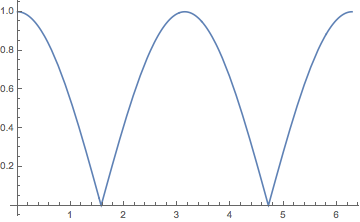
\includegraphics[scale=0.5]{cos_abs} & 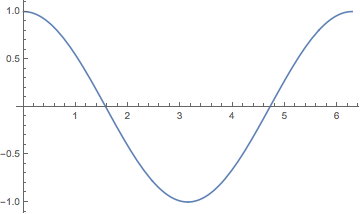
\includegraphics[scale=0.5]{cos}\\
$f(x) = |\cos{x}|$ on $[0,2\pi]$ & $f(x) = \cos{x}$ on $[0,2\pi]$
\end{tabular}
\end{center}
\noindent\\ You can see that the section of the graph from
$[\frac{\pi}{2},\frac{3 \pi}{2}]$ is positive for the $|\cos{x}|$, but negative
for $\cos{x}$. If we simply integrated the $|\cos{x}|$ over $[0,\pi]$, the
result would be 0, but graphically this result would not make any sense. Now
let's take a look at the $b_{n}$ term. Before we jump into the integration,
let's think about this function:
\[\left|\cos{x}\right| =
\begin{cases*}
\cos(x) \qquad 0\leq x \leq \frac{\pi}{2}\\
-\cos(x)\quad  \frac{\pi}{2}\ \leq x \leq \pi
\end{cases*}
\]
\noindent Now we can set up the formula for the $b_{n}$ term. We have as follows:
\begin{align*}
b_{n} &= \frac{2}{\pi}\left[ \int_{0}^{\frac{\pi}{2}} \cos{x}\cos{nx}dx - \int_{\frac{\pi}{2}}^{\pi} \cos{x}\cos{nx}dx \right]\\
&= \frac{2}{\pi} \left[ \frac{-2 \cos{\left(\frac{n\pi}{2}\right)} + \sin{\left(n\pi\right)}}{n^{2} - 1}\right]\\
\end{align*}
\noindent Note that (as we have seen before) the sine term disappears; however,
the more interesting part is what happens with our cosine term. The value of
$\cos{\left(\frac{n\pi}{2}\right)}$ will be 0 at all odd $n$, or for all
$n = 2k + 1$. So, we will let our $n = 2k$. This gives us:
\begin{align*}
b_{n} &= \frac{2}{\pi} \left[ \frac{-2 \cos{\left(k \pi \right)}}{(2k)^{2} - 1}\right]\\
&= -\frac{4}{\pi}\left[\frac{(-1)^{k}}{(2k)^{2}-1}\right]
\end{align*}
\noindent And that leaves us with the final result
\[
f(x)\sim \frac{2}{\pi} - \sum_{k=0}^{\infty}\left[\frac{4}{\pi}\left[\frac{(-1)^{k}}{(2k)^{2}-1}\right]
\cos{\left(\frac{2k\pi}{2}\right)}\right]
\]
And we are done.
\newpage



\subsection{Convergence of Fourier Series}
\indent Up to this point, we have found a Fourier series and left our solutions
at that. We will now look into the convergence of a Fourier series. This topic
includes two questions:
\begin{enumerate}
\item Does the series converge?
\item If the series converges, to what value does it converge?
\end{enumerate}
\noindent Before we jump into convergence, we need to review some ideas.
\begin{enumerate}
\item \textit{\textbf{Jump Discontinuity:}} To say that $f(x)$ has a jump
discontinuity at $x = a$ is to say that
\[
\lim_{x \to a^{-}}f(x) \neq \lim_{x \to a^{+}}f(x)
\]
Where both the limit from the left and the limit from the right exist.
\item \textit{\textbf{Piecewise Smooth:}} A function $f(x)$ is said to be
piecewise smooth if the function can be broken into two distinct intervals, and
on each interval both $f(x)$ and $f^{'}(x)$ are continuous.
\item \textit{\textbf{Periodic Extension:}} The periodic extension of $f(x)$ on
$[-L,L]$ is the repetition of the function on intervals on periods to the left
and right of $[-L,L]$.
\end{enumerate}
\indent With these definitions, we can lay out a general rule for convergence of
a Fourier series. We won't give a proof of these rules for the time being. We
just need them to lay out some groundwork for the rest of the information we
will present on Fourier series. We have the following:
\begin{quote}
Suppose $f(x)$ is a function, and that $f(x)$ is piecewise smooth on the interval
$[-L,L]$. The corresponding Fourier series for $f(x)$ converges to either
\begin{enumerate}
\item the periodic extension of $f(x)$, if $f(x)$ is continuous, or
\item the average of the two one-sided limits, if the periodic extension of
$f(x)$ has a jump discontinuity at $x = a$.
\end{enumerate}
\end{quote}
\noindent We should note that the second condition can be expressed by the formula
\[\frac{1}{2}\left[\lim_{x \to a^{-}}f(x) + \lim_{x \to a^{+}}f(x)\right]\]
which gives us a nice way to calculate the value to which the series converges
if we happen to meet the criteria in (2). Let's take a look at some examples.\\\\


\noindent\textbf{\textit{Ex:}} Find the Fourier series for the following
equation, and determine if the series converges. If it does, tell where the
series will converge.
\[ f(x) =
\begin{cases}
L \qquad\qquad -L \leq x \leq 0\\
2x \qquad\qquad 0 \leq x \leq L
\end{cases}
\]
\indent\textbf{\textit{Solution:}} We will go ahead and skip the details of
finding the Fourier series for this function. If you do want to find it, you
will have to find a full piecewise Fourier series. For this particular $f(x)$,
we have:
\begin{align*}
f(x) &\sim L + \sum_{n=1}^{\infty}\left[\frac{2L}{n^{2}\pi^{2}}([-1]^{n}-1)\cos{\left(\frac{n\pi
x}{L}\right)}\right] - \sum_{n=1}^{\infty}\left[\frac{L}{n\pi}(1 + [-1]^{n})\sin{\left(\frac{n\pi
x}{L}\right)}\right]
\end{align*}
\noindent Notice that we didn't simplify this solution to a nicer form.
If we evaluate this series, we will run across terms where the series is 0, but
that is okay for now. This function is also defined as a piecewise function,
and on both intervals ($[-L,0]$ and $[0,L]$), $f(x)$ is continuous. In other
words, $f(x)$ is piecewise smooth, so we know that this series converges. Now
let's take a look at the graph of $f(x)$ on an arbitrary interval of $[-1,1]$.
\begin{center}
\begin{tabular}{c}
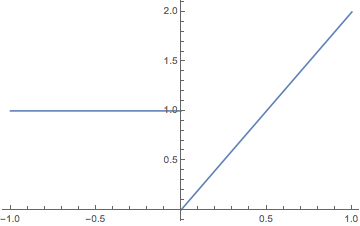
\includegraphics[scale=0.6]{pw_graph_01}\\
$
f(x) =
\begin{cases}
1 \qquad\qquad -1 \leq x \leq 0\\
2x \qquad\qquad 0 \leq x \leq 1
\end{cases}
$
\end{tabular}
\end{center}
\noindent We can see that there is a jump in the graph at $x = 0$. In other
words, there is a jump discontinuity at $x = 0$, and that means that we need to
use (2) in order to find the value of convergence. We will let $\sum$ stand in
for our entire series. We have:
\begin{align*}
\sum &\to \frac{1}{2}\left[\lim_{x\to 0}L + \lim_{x\to0}2x\right]\\
&\to \frac{1}{2}[L + 0]\\
&\to \frac{L}{2}
\end{align*}
\noindent So, at $x=0$, the series converges to $\frac{L}{2}$. We are not done
yet, however. Now, we need to consider the periodic extension of the series. The
function will repeat every $[-L,L]$, so we need to look at what the convergence
of the series looks like at $-L$ and $L$. Let's take a look:
\begin{alignat*}{3}
\sum&\to\frac{1}{2}\left[\lim_{x\to-L^{-}}f(x) + \lim_{x\to-L^{+}}f(x)\right] \qquad\qquad \sum&&\to
\frac{1}{2}\left[\lim_{x\to L^{-}}f(x) + \lim_{x\to L^{+}}f(x)\right]\\
&\to \frac{1}{2}[2L + L] &&\to \frac{1}{2}[2L + L]\\
&\to\frac{3L}{2} &&\to\frac{3L}{2}
\end{alignat*}
\noindent And we are done.
\newpage



\section{Second Order Partial Differential Equations}
\hrule
\noindent\\
\subsection{The Heat and Wave Equations}
\indent Let's take a look at the second order PDE. We will start with a
homogeneous equation, which we will tackle with the separation of variables
method. The general strategy is that we want to take our PDE and convert it to
an ODE, which we know how to solve. The problems presented here also involve
boundary conditions, which will require us to solve for eigenvalues/functions.
We will also be dealing with series (specifically Fourier Series) to help us
solve these problems. Let's look at an example:\\

\newpage
\noindent\textbf{\textit{Ex:}} Solve the following boundary value problem:
\[
\begin{cases}
u_{tt} - u_{xx} = 0\\
u(0,t) = 0\qquad u(1,t) = 0\\
u(x,0) = f(x)\qquad u_{t}(x,0) = g(x)
\end{cases}\\
\]
\[f(x) = 2\sin{(\pi x)} + 3\sin{(2\pi x)}\qquad g(x) = 4\sin{(3\pi x)} - 7\sin{(5\pi x)}\]
given the general solution:
\[u(x,t) = \sum_{n=1}^{\infty}\left[\left(a_{n}\cos{[n\pi t]} + b_{n}\sin{[n\pi t]}\right)\sin{[n\pi
x]}\right]\]
\indent\textbf{\textit{Solution:}} There's a lot going on here, so let's break
it down. First of all, notice that we have two initial conditions, one of which
is a derivative. This should make sense since the equation have two second order
partial derivatives included in it. Next notice that we have a Fourier Sine Series,
despite both the $\sin{[n\pi t]}$ and $\cos{[n\pi t]}$ terms. If we had worked
out the entire problem, we would see that our eigenvalue/function for this
equation takes the form of
\[
\{\lambda_{n} = n\pi, \sin{(n\pi x)}\}
\]
\noindent which tells us that the corresponding series is a Fourier Sine Series.
We also see the initial conditions on our equation are already representative
of a series of sine functions, which is not just a conincidence. To apply the
initial conditions, we will need both the general solution and the derivative
with respect to $t$ of the general solution. Let's go ahead and apply the first
initial condition, $u(x,0) = f(x)$. Letting $t= 0$ gives us:
\[
u(x,0) = 2\sin{(\pi x)} + 3\sin{(2\pi x)} = \sum_{n=1}^{\infty}\left[a_{n}\sin{(n\pi x)}\right]
\]
\noindent We see that the term with $b_{n}$ has dropped out, since
$\sin{(0)} = 0$. Now we just have to match up the coefficients on $a_{n}$. We
can see that when we have $n=1$, $a_{n} = 2$, and when $n=2$, $a_{n} = 3$. For
all other $n$, we have $a_{n} = 0$, so we ignore those terms. Next, we can apply
the initial condition for the derivative of the general solution with respect to
$t$. We expect that all the terms related to $a_{n}$ will disappear, and in fact
they will. Let's take a look:
\begin{align*}
u_{t}(x,t) &= \sum_{n=1}^{\infty}\left[(-a_{n}n\pi\sin{[n\pi t]} + b_{n}n\pi\cos{[n\pi t]})\sin{n\pi
x}\right]\\
u_{t}(x,0) &= 4\sin{(3\pi x)} - 7\sin{(5\pi x)} = \sum_{n=1}^{\infty}\left[n\pi b_{n}\sin{(n\pi
x)}\right]
\end{align*}
\noindent We are going to do the same thing here that we did to find our $a_{n}$
terms, but notice that we don't just have $b_{n}$; we actually have $n\pi b_{n}$.
We have the following:
\begin{alignat*}{3}
&3\pi b_{3} = 4 \qquad \qquad \qquad &&5\pi b_{5} = -7\\
&b_{3} = \frac{4}{3\pi} &&b_{5} = -\frac{7}{5\pi}
\end{alignat*}
\noindent Much like the solutions for $a_{n}$, all the other $b_{n}$ terms are 0.
Now we can construct a particular solution. In this case, the answer will not be
in the form of a series, since we have definite terms. Our solution is as follows:
\[
u(x,t) = 2\cos{(\pi t)}\sin{(\pi x)} + 3\cos{(2\pi t)}\sin{(2\pi x)} + \frac{4}{3\pi}\sin{(3\pi
t)}\sin{(3\pi x)} - \frac{7}{5\pi}\sin{(5\pi t)}\sin{(5\pi x)}
\]
\noindent And we are done.
\newpage

\noindent \textbf{\textit{Ex:}} Solve the following PDE
\[
\begin{cases}
\frac{\partial u}{\partial t} = k \frac{\partial^{2} u}{\partial x^{2}}\\
u(x,0) = x\\
u(0,t) = u(L,t) = 0\\
\end{cases}
\]
\indent \textbf{\textit{Solution:}} We will use the separation of variable
technique to solve this problem. We know to use separation of variable because
we are dealing with a homogeneous PDE with homogenous boundary conditions.
Separation of variables tells us that our solution will be in the form of
$u(x,t) = X(x)T(t)$. If we take this fact at face value, we can use the
separation of variables method to solve this. First, we substitute in our solution
into the PDE:
\begin{align*}
\frac{\partial}{\partial t}(X(x)T(t)) &= k \frac{\partial^{2}}{\partial x^{2}}(X(x)T(t))\\
X(x)\frac{dT}{dt} &= k\frac{d^{2}X}{dx^{2}}T(t)\\
\frac{dT}{dt}\frac{1}{T(t)} &= \frac{d^{2}X}{dx^{2}}\frac{k}{X(x)}
\end{align*}
\noindent The only way that our function of x and our function of t can be equal
is if they are equal to a constant; thus we now have:
\[
\frac{dT}{dt}\frac{1}{T(t)} = \frac{d^{2}X}{dx^{2}}\frac{k}{X(x)} = -\lambda
\]
\noindent And now we have a first order ODE for the time and a second order ODE
for the position:
\[
\frac{dT}{dt} = -k \lambda T(t) \qquad\text{and}\qquad \frac{d^{2}X}{dx^{2}} = -\lambda X(x)
\]
\noindent Our next step is to find the Eigenvalues and Eigenfunctions of the
second order ODE; we will come back to the time ODE when we have values for
$\lambda$.\\
\indent To solve for these values, we have to find non-trivial eigenvalues that
correspond to the boundary values of the ODE. In this case, we know that
$X(0) = 0$ and $X(L) = 0$. These boundary conditions come from the BC on the PDE
which states $u(0,t) = u(L,t) = 0$. To find the eigenvalues/functions, we need
to find the characteristic equation corresponding to the ODE in question. Let's
go ahead and find it:
\begin{gather*}
\frac{d^{2}X}{dx^{2}} = -\lambda \frac{X(x)}{k}\\
\frac{d^{2}X}{dx^{2}}  + \lambda \frac{X(x)}{k} = 0\\
r^{2} + \lambda = 0\\
r^{2} = -\lambda\\
r = \pm \sqrt{- \lambda}
\end{gather*}
\indent Now, we can substitute values of $\lambda$ to find out solutions. Let's
start with $\lambda > 0$. Since we have a $-\lambda$ under the radical, we will
have $r = \pm \sqrt{\lambda} \mathrm{i}$. This will yield the solution of
\[
y(x) = c_{1}\cos{\sqrt{\lambda}x} + c_{2}\sin{\sqrt{\lambda}x}
\]
\noindent Applying our boundary conditions gives us:
\[
y(0) = c_{1}\cos{0} + c_{2}\sin{0} = 0
\]
\noindent Now we know that $c_{1} = 0$. This result came from the fact that
$\sin{0} = 0$, so the $c_{2}$ term disappears. Now we are left with $\cos{0} = 1$,
which tells us that $c_{1} = 0$. We can apply this to our second boundary
condition like so:
\begin{gather*}
y(L) = 0 = c_{2}\sin{\sqrt{\lambda}L}\\
\end{gather*}
\noindent It looks like there will only be trivial solutions, but we know this
isn't true due to the Jacobian matrix. Recall that if the determinant of the
Jacobian $\neq 0$, then we only have trivial solutions, and if the determinant
of the Jacobian $= 0$, then we do not have the trivial solution. Let's take a
look at the Jacobian for this case:
\begin{gather*}
\left|
\begin{array}{cc}
1 & 0\\
\cos{\sqrt{\lambda}L} & \sin{\sqrt{\lambda}L}
\end{array}
\right| = 0\\
\sin{\sqrt{\lambda}L} = 0\\
\sqrt{\lambda}L = \arcsin{0}\\
\sqrt{\lambda} = \frac{\arcsin{0}}{L}\\
\lambda = \left(\frac{\arcsin{0}}{L}\right)^{2}\\
\lambda = \left(\frac{n\pi}{L}\right)^{2}
\end{gather*}
\noindent Notice that we replaced the $\arcsin{0}$ term with $n\pi$. Recall from
trig that the $\sin$ function is $0$ at every $n\pi$, starting with $n = 0$.
Next, we just need to find our corresponding eigenfunction. Our $c_{1}$ was $0$,
so we can ignore the entire $\cos$ term. Thus, we have an eigenfunction from
plugging in our $\lambda$ that looks like:
\[
X(x) = \sin{\frac{n\pi x}{L}}
\]
\indent Unfortunately, we aren't done yet. Now we have to find the corresponding
eigenvalues/functions for $\lambda = 0$. This isn't too hard, and can be done in
a few lines if we recall the characteristic equation. Plugging in $0$ for
$\lambda$ gives us that $r = 0$. Using this piece of information, we now know
that $y(x) = c_{1} + xc_{2}$. Applying our boundary conditions gives us
$c_{1} = 0, c_{2} = 0$. We can see that we have only trivial solutions for
$\lambda = 0$.\\
\indent Our final case is for $\lambda < 0$. I'll go ahead and tell you that
this will yield another trivial solution, but we can take a look at the work
behind it. Since $\lambda > 0$, we know that our $r$ from the characteristic
equation will be $r = \pm \sqrt{\lambda}$. From here we are going to do something
 a little unconventional that will help us. Usually, we would have a solution of
the form $y(x) = c_{1}e^{\sqrt{\lambda}x} + c_{2}x e^{-\sqrt{\lambda}x}$. In our
case, it will be more convenient to use hyperbolic trig functions. It's not too
far off from our solution from $\lambda > 0$:
\begin{align*}
y(x) &= c_{1}e^{\sqrt{\lambda}x} + c_{2}e^{-\sqrt{\lambda}x}\\
&= c_{1}\cosh{\sqrt{\lambda}x} + c_{2}\sinh{\sqrt{\lambda}x}
\end{align*}
\noindent If we apply the boundary conditions (remember that
$\sinh{0} = 0$ and $\cosh{0} = 1$), we will find that we have only trivial
solutions.\\
\indent So, we are done with the second order ODE, and now we turn our eye to
the first order time equation. We know our $\lambda$, so it isn't too hard to solve:
\begin{gather*}
\frac{dT}{dt} = -\lambda T(t)\\
T(t) = ce^{-k\left(\frac{n\pi}{L}\right)^{2}t}
\end{gather*}
\indent Finally we can put it all together. Our penultimate solution will be
\[
u_{n}(x,t) = B_{n}\sin{\left(\frac{n\pi x}{L}\right)}e^{-k\left(\frac{n\pi}{L}\right)^{2}t}
\]
\noindent We can analyze this solution and tell where each piece comes from.
The $B_{n}$ is a coefficient that results from our $c's$ in the general solutions
of the differential equations. The $sin$ part results from out eigen vector.
Remember, we get a different value for each $n$, so there may or may not be $0$
terms in the series. Finally, we have the exponential term. This term comes from
the solution to our time equation. When we put it all together, we can see that
this is, of course a series; for every $n$, we get a different solution. From
here we can find the Fourier Series (which will be a Fourier Sine Series). We
won't worry about that yet, but we will come back to it.
\newpage


\indent It will benefit us to take a moment and discuss how boundary conditions
effect our Fourier series. We have three different combinations of boundary
conditions, where each one will produce a different result in our series solution.
\begin{enumerate}
\item \textit{Dirichlet Boundary Conditions}\\
Dirichlet boundary conditions involve the function for which we are looking. In
other words, the boundary conditions are presented in terms of the functions we
are trying to find, rather than the derivative of that function. Typically, this
type of boundary condition will take the form of (in the homogeneous case)
\[u(0,t) = u(L,t) = 0.\]
In regards to our Fourier series, we expect to see $\sin{(\frac{n\pi x}{L})}$.
Our basis will look like
\[
\left\{ \lambda_{n} = \left(\frac{n\pi}{2}\right)^{2}, \phi_{n}(x) = \sin{\left(\frac{n\pi x}{L}\right)} \right\}
\]
\item \textit{Neumann Boundary Conditions}\\
Neumann boundary conditions involve the derivatives of the function for which we
are solving. Neumann boundary conditions will look like
\[u_{x}(0,t) = u_{x}(L,t) = 0.\]
This will cause our Fourier series to contain $\cos{(\frac{n\pi x}{L})}$. Our
basis will look like
\[
\left\{ \lambda_{n} = \left(\frac{n\pi}{2}\right)^{2}, \phi_{n}(x) = \cos{\left(\frac{n\pi x}{L}\right)} \right\}
\]
\item \textit{Robin Boundary Conditions}\\
Robin boundary conditions will contain a mixture of the function and it's
derivative. Typically, we will see
\[ u_{x}(0,t) = u(L,t) = 0\qquad \text{or}\qquad u(0,t) = u_{x}(L,0) = 0.\]
These boundary conditions will give us two different results, depending on whether
we have the derivative first or second. We will have
\begin{align*}
u_{x}(0,t) = u(L,t) = 0 &\implies \left\{\lambda_{n} = \left(\left[n + \frac{1}{2}\right]\frac{\pi}{L}\right)^{2}, \phi_{n}(x) = \cos{\left(\left[n + \frac{1}{2}\right]\frac{\pi}{L}x\right)}\right\}\\
u(0,t) = u_{x}(L,t) = 0 &\implies \left\{\lambda_{n} = \left(\left[n + \frac{1}{2}\right]\frac{\pi}{L}\right)^{2}, \phi_{n}(x) =\sin{\left(\left[n + \frac{1}{2}\right]\frac{\pi}{L}x\right)}\right\}
\end{align*}
\end{enumerate}

\indent Now we can take a look at a slightly harder PDE. We still have the heat
equation, but we will not have homogeneous boundary conditions. Our goal here is
to find a way to transform our boundary conditions into a homogenous form and take
it from there.\\\\
\noindent \textbf{\textit{Ex:}} Solve the following PDE
\[
\begin{cases*}
u_{t} - u_{xx} = 0\\
u(0,t) = 0,\ u(1,t) = t\\
u(x,0) = x^{2}
\end{cases*}
\]
\indent \textbf{\textit{Solution:}} We would like to just jump into this PDE and
solve it, but it's not quite that simple. We have to find a way to express our
boundary conditions in a homogeneous manner. We can do this through a clever
substitution; we will create a new PDE, denoted $\Upsilon$. To find $\Upsilon$,
we use the following formula:
\[ \Upsilon = B_{1} + \frac{x}{l}\Delta B, \]
\noindent where $B$ is a boundary condition. In our case, we have as follows:
\begin{align*}
\Upsilon &= B_{1} + \frac{x}{l}\Delta B\\
&= 0 + \frac{x}{1}(t - 0)\\
&= xt
\end{align*}
\noindent Now, we find a new PDE, denoted by $\upsilon$. We have another formula that tells us
\[ \upsilon(x,t) = u(x,t) - \Upsilon(x,t) \]
\noindent Applying this formula gives us
\begin{align*}
\upsilon(x,t) &= u(x,t) - \Upsilon\\
&= u(x,t) - xt
\end{align*}
\noindent Let's take a moment to analyze the result. We wanted to find a new PDE in terms of our old one that would allow us to have homogeneous boundary conditions. We found a solution, called $\upsilon$, in terms of our original PDE, called $u$. Our original PDE was $u_{t} - u_{xx} = 0$, so to properly perform our substitution, we need to find $\upsilon_{t}$ and $\upsilon_{xx}$. Through some careful differentiation, we have
\[ \upsilon_{t} = u_{t} - x \qquad\text{and}\qquad \upsilon_{xx} = u_{xx}\]
\noindent To find our new PDE, we simply evaluate.
\[
\upsilon_{t} - \upsilon_{xx} = u_{t} - x - u_{xx} = u_{t} - u_{xx} - x = 0 - x = -x
\]
\noindent So we finally have a new PDE that looks like
\[
\begin{cases*}
\upsilon_{t} - \upsilon_{xx} = -x\\
\upsilon(0,t) = \upsilon(1,t) = 0\\
\upsilon(x,0) = x^{2}
\end{cases*}
\]
\noindent You may wonder how this has made anything simpler, since the PDE itself is no longer homogeneous. By forcing the boundary conditions to be homogeneous, we can now use a Fourier series to find our solution. Recall that earlier we discussed the boundary condition and their resulting eigenvalue/eigenfunction. Here, we have Dirichlet boundary conditions, which tells us that we have a Fourier sine series. We have that
\begin{align*}
\upsilon(x,t) &= \sum_{n = 1}^{\infty}\left[a_{n}(t)\sin{(n\pi x)}\right]\\
\upsilon_{t}(x,t) &= \sum_{n = 1}^{\infty}\left[a_{n}'(t)\sin{(n\pi x)}\right]\\
\upsilon_{xx}(x,t) &= -\sum_{n = 1}^{\infty}\left[a_{n}(t)(n\pi)^{2}\sin{(n\pi x)}\right]\\
\end{align*}
\noindent Which tells us that
\[
\upsilon_{t} - \upsilon_{xx} = \sum_{n = 1}^{\infty}\left[(a_{n}'(t) + (n\pi)^{2}a_{n}(t))\sin{(n\pi x)}\right] = -x
\]
\noindent This may look rather complicated, but all we have is a function's Fourier sine series. Essentially, we have
\[
-x = \sum_{n = 1}^{\infty}\left[ b_{n}\sin{(n\pi x)} \right]
\]
\noindent To find $b_{n}$, we use the formula that was discussed in the earlier section about Fourier series. We have that
\begin{align*}
a_{n}'(t) + (n\pi)^{2}a_{n}(t) &= \int_{0}^{1}-x\sin{(n\pi x)}dx\\
&= \frac{2x}{n\pi}\cos{(n\pi x)}\bigg\vert_{0}^{1}\\
&= \frac{2}{n\pi}
\end{align*}
\noindent We now have an ODE which we can solve for $a_{n}$. Note that from out PDE, we do have an initial condition for the ODE, but it is not as simple as just saying $a_{n}(0) = x^{2}$. At $t = 0$, we have the following series:
\[
\sum_{n=1}^{\infty} a_{n}(0)\sin{(n\pi x)}
\]
\noindent We got this by taking our original $\upsilon(x,t)$ and plugging in $0$ for $t$. We know how to get $a_{n}(0)$, since this is just a simple Fourier sine series. It is given by
\begin{align*}
a_{n}(0) &= 2\int_{0}^{1}x^{2}\sin{(n\pi x)}dx\\
&= \frac{(-1)^{(n + 1)}}{n\pi} + \frac{2}{(n\pi)^{3}}\left[ (-1)^{n} - 1 \right]
\end{align*}
\noindent We now have all we need to solve the ODE. We will omit the work for the solution, but the final answer for $a_{n}$ is
\[
a_{n}(t) = \frac{4\left[ (-1)^{n} - 1 \right]}{(n\pi)^{3}}e^{-(n\pi)^{2}t} + \frac{2(-1)^{n}}{(n\pi)^{3}}
\]
\noindent Now all that's left to do is go back to $u$ from $\upsilon$. This may seem hard, but we saw earlier that $\upsilon = u - \Upsilon$. Solving for $u$ gives us $u = \upsilon + \Upsilon$. Recall that $\Upsilon$ was $xt$, and $\upsilon$ was the series for which we just found $a_{n}$. Putting it all together gives us
\[
u(x,t) = xt + \sum_{n=1}^{\infty}\left[\frac{4\left[ (-1)^{n} - 1 \right]}{(n\pi)^{3}}e^{-(n\pi)^{2}t} + \frac{2(-1)^{n}}{(n\pi)^{3}}\right]\sin{(n\pi x)}
\]
\noindent And we are done.
\newpage


\noindent \textbf{\textit{Ex:}} Solve the following PDE
\[
\begin{cases*}
u_{tt} - u_{xx} = 1 + t\cos{(2\pi x)}\\
u_{x}(0,t) = u_{x}(1,t) = 0\\
u(x,0) = 2\cos{(2\pi x)},\quad u_{t}(x,0) = 1 + \cos{(\pi x)} - \cos{(2\pi x)}
\end{cases*}
\]
\indent \textbf{\textit{Solution:}} This problem is an example of the wave equation with a non-homogeneous solution. We are lucky this time; the boundary conditions are already homogeneous, so there is no need to change our variable. We know that since both of the boundary conditions are derivatives, we are dealing with a Fourier cosine series. This yields the eigenvalue/function of
\[
\left\{\lambda_{n} = (n\pi)^{2}, \cos{(n\pi x)}\right\}
\]
Since we are dealing with a cosine series, we also have a leading term, $a_{0}$. Our full series looks like
\[
u(x,t) = a_{0}(t) + \sum_{n=1}^{\infty} a_{n}(t)\cos{(n\pi x)}
\]
We need $u_{tt}$ and $u_{xx}$, so we have:
\[
u_{tt}(x,t) = a_{0}''(t) + \sum_{n=1}^{\infty} a_{n}''(t)\cos{(n\pi x)}
\qquad \text{and} \qquad
u_{xx}(x,t) = -\sum_{n=1}^{\infty} (n\pi)^{2}a_{n}(t)\cos{(n\pi x)}
\]
All we have to do now is simply plug into our original equation. This gives us
\begin{align*}
a_{0}''(t) + \sum_{n=1}^{\infty} a_{n}''(t)\cos{(n\pi x)} + \sum_{n=1}^{\infty} (n\pi)^{2}a_{n}(t)\cos{(n\pi x)} &= 1 + t\cos{(2\pi x)}\\
a_{0}''(t) + \sum_{n=1}^{\infty}(a_{n}''(t) + (n\pi)^{2}a_{n}(t))\cos{(n\pi x)} &= 1 + t\cos{(2\pi x)}
\end{align*}
Now we can play the matching game. We have a $constant + series\ term$ on the right side, and $constant + series$ on the left, so we can match up the constants. This gives us
\[
a_{0}''(t) = 1
\]
Now we match up the series term. On the right hand side, we have $\cos{(2\pi x)}$, so we know that for $n= 2$, we have
\[
a_{2}''(t) + 4\pi^{2}a_{2}(t) = t
\]
$a_{0}$ and $a_{2}$ are the only terms that appear, so we can assume for now that $\forall n \neq 2\ \text{and}\ 3, a_{n} = 0$. We are left with two ODE's, so we now need to find the corresponding initial conditions. Let's apply the first initial condition to our PDE. This gives us
\[a_{0}(0) + \sum_{n=1}^{\infty}a_{n}(0)\cos{(n\pi x)} = 2\cos{(2\pi t)}\]
Which tells us
\[a_{0} = 0 \qquad\qquad \qquad\qquad a_{2} = 2\]
Now we can apply the second initial condition. After taking the partial derivative of $u$ with respect to $t$, we have
\[
a_{0}'(0) + \sum_{n=1}^{\infty}a_{n}'(0)\cos{(n\pi x)} = 1 + \cos{(\pi x)} - \cos{(2\pi x)}
\]
Some more clever pattern matching give us
\[
a_{0}'(0) = 1 \qquad\qquad a_{1}'(0) = 1 \qquad\qquad a_{2}'(0) = -1
\]
Notice that we have a term $a_{1}'$. We cannot simply ignore this value; rather we have to take it into account when we find our solution. We know that we have an ODE for $a_{1}(t)$, but it may not be evident how to express it. Recall that earlier we said $\forall n \neq 2\ \text{and}\ 3, a_{n} = 0$. This means that $a_{1} = 0$, and since $a_{1}$ is a coefficient in the Fourier series, we know that $a_{1}''(t) + \pi^{2}a_{1}(t) = 0$. We now have three different ODE's that we must solve:
\begin{alignat*}{3}
&\begin{cases}
a_{0}''(t) = 1\\
a_{0}'(0) = 1,\quad a_{0}(0) = 1
\end{cases}
&\begin{cases}
a_{1}''(t) + \pi^{2}a_{1}(t) = 0\\
a_{1}'(0) = 1,\quad a_{1}(0) = 0
\end{cases}
&&\begin{cases}
a_{2}''(t) + 4\pi^{2}a_{2}(t) = t\\
a_{2}'(0) = 1,\quad a_{2}(0) = 2
\end{cases}
\end{alignat*}
Luckily, Mathematica is here to save the day. We will skip the work and let the computer do the thinking for us. We get that
\begin{align*}
a_{0}(t) &= \frac{1}{2}t^{2} + t\\
a_{1}(t) &= \frac{\pi\cos{(t\pi)} + \sin{(t\pi)}}{\pi}\\
a_{2}(t) &= \frac{2\pi t + 16\pi^{3}\cos{(2\pi t)} - \sin{(2\pi t)} + 4\pi^{2}\sin{(2\pi t)}}{8\pi^{3}}
\end{align*}
Now all we need to do is plug back in to our $u$. Our final answer becomes
\[
u(x,t) = \frac{1}{2}t^{2} + t + \frac{\pi\cos{(t\pi)} + \sin{(t\pi)}}{\pi}\cos{(\pi x)} +  \frac{2\pi t + 16\pi^{3}\cos{(2\pi t)} - \sin{(2\pi t)} + 4\pi^{2}\sin{(2\pi t)}}{8\pi^{3}}\cos{(2\pi x)}
\]
Just for interest, the plot of this solution looks like
\begin{center}
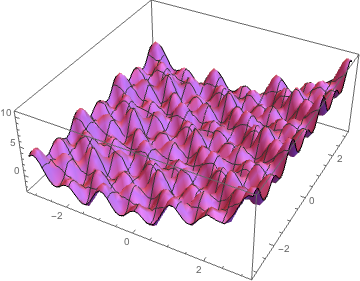
\includegraphics[scale=0.6]{pg23_plot}
\end{center}
On $-\pi \leq \theta \leq \pi$ and $-\pi \leq x \leq \pi$; and we are done.
\newpage


\subsection{The Laplace Equation}
\noindent \\
\indent Up to this point, we have only looked at the wave equation and the heat equation. There is, however, one other equation in the classical trinity: the Laplace Equation. We haven't dealt with this equation yet because we have to be very careful in our approach to solving it. When we looked at the homogeneous wave and heat equations, we used the general approach called \textit{Separation of Variables}. In the case of the homogeneous Laplace equation, we may not be able to tackle the problem using separation of variables. The problem arises from the various types of boundaries that effect the domain. We can either have a 'rectangular' bound, which will be separable, or a 'circular' bound which is \textbf{not} separable. Imagine that we have the following two problems:
\begin{align*}
&A =\begin{cases}
u_{xx} + u_{yy} = 0\quad \text{on}\ [0,1]\times[0,2]\\
u(x,0) = u(x,2) = 0\\
u(0,y) = y, u(1,y) = 0
\end{cases}
&B =\begin{cases}
u_{xx} + u_{yy} = 0\quad \text{on}\ x^{2} + y^{2} < a^{2}\\
u(x,y)\ \big |_{x^{2} + y^{2} = a^{2}} = f(x,y)
\end{cases}
\end{align*}
$A$ is an example of a separable Laplace equation. We can see graphically that the domain $[0,1] \times [0,2]$ is rectangular. $B$'s domain is not separable, since it is circular. Let's take a look at $A$.\\\\
\noindent \textbf{\textit{Ex:}} Solve the following PDE
\[
\begin{cases*}
u_{xx} + u_{yy} = 0\quad \text{on}\ [0,1]\times[0,2]\\
u(x,0) = u(x,2) = 0\\
u(0,y) = y, u(1,y) = 0
\end{cases*}
\]
\indent \textbf{\textit{Solution:}} Earlier, we discussed the different boundary conditions we can encounter and their corresponding eigenvalues/functions. In this problem, we have Dirichlet boundary conditions. This tells us that
\[
\left\{\lambda_{n} = \left(\frac{n\pi}{2}\right)^{2}, \phi_{n}(y) = \sin{\left(\frac{n\pi y}{2}\right)}\right\}
\]
Notice that we used $y$ here instead of $x$. We did this because the boundary conditions are defined in terms of $y$, not $x$. Now we can continue to solve our problem. Recall that our separation of variables gives us two second order ODE's,
\[
X'' - \lambda X = 0 \qquad\qquad \text{and} \qquad\qquad \lambda Y - Y'' = 0
\]
We already solved for $Y(y)$ by finding the corresponding eigenvalues/vectors. Now we plug in our $\lambda_{n}$ into our $X$ ODE. Solving the resulting ODE will give us a basis of
\[
\left\{ e^{\frac{n\pi}{2}x}, e^{-\frac{n\pi}{2}x} \right\}
\]
Now we could continue at this point, but if we think ahead, we can see that when we eventually apply our initial conditions, nothing will cancel out. At this point, we want to transform our basis. We have as follows
\[
\left\{ e^{\frac{n\pi}{2}x}, e^{-\frac{n\pi}{2}x} \right\} \implies \left\{ \cosh{\left(\frac{n\pi x}{2}\right)}, \sinh{\left(\frac{n\pi x}{2}\right)} \right\}
\]
All we did here is apply an identity. Now we have everything we need to set up a solution. Our $u(x,y)$ will be
\[
u(x,y) = \sum_{n=1}^{\infty}\left[a_{n}\cosh{\left(\frac{n\pi x}{2}\right)} + b_{n}\sinh{\left(\frac{n\pi x}{2}\right)}\right]\sin{\left(\frac{n\pi y}{2}\right)}
\]
We can apply our initial conditions, which gives us $b_{n}\ \text{and}\ a_{n}$:
\begin{align*}
a_{n} &= \frac{4(-1)^{n+1}}{n\pi}\\
b_{n} &= -\coth{\left(\frac{n \pi}{2}\right)}\frac{4(-1)^{n+1}}{n\pi}
\end{align*}
This yields a final solution of
\[
u(x,y) = \sum_{n=1}^{\infty}\left[ \frac{4(-1)^{n+1}}{n\pi} \cosh{\left(\frac{n\pi x}{2}\right)} -\coth{\left(\frac{n \pi}{2}\right)}\frac{4(-1)^{n+1}}{n\pi}\sinh{\left(\frac{n\pi x}{2}\right)}\right]\sin{\left(\frac{n\pi y}{2}\right)}
\]
And we are done
\newpage


\indent Now we turn our attention to the Laplace Equation with a circular domain. As we discussed earlier, we can't simply say that our solution will be in the form of $X(x)Y(y)$. However, we can force the domain to be rectangular if we use polar coordinates. Let's consider a variation of $B$ from above.\\\\

\noindent \textbf{\textit{Ex:}} Solve the following PDE
\[
\begin{cases*}
u_{xx} + u_{yy} = 0\quad \text{on}\ x^{2} + y^{2} < a^{2}\\
u(a,\theta) = U_{1}\quad \text{on}\ 0 \leq \theta \leq \pi\\
u(a,\theta) = U_{2}\quad \text{on}\ \pi \leq \theta \leq 2\pi
\end{cases*}
\]
\indent \textbf{\textit{Solution:}} We want to express the partial derivatives here in terms of $r\ \text{and}\ \theta$. Recall that we have
\[
x = r\cos{\theta} \qquad\qquad \text{and} \qquad\qquad y = r\sin{\theta}
\]
First, we will find the partial derivatives of $x$ and $y$ with respect to $r$ and $\theta$. Since $x = r\cos{\theta}$,
\[
\frac{\partial x}{\partial r} = \cos{\theta} \qquad\qquad \frac{\partial x}{\partial \theta} = -r\sin{\theta}
\]
We can compute the derivatives for $y$ in a similar fashion:
\[
\frac{\partial y}{\partial r} = \sin{\theta} \qquad\qquad \frac{\partial y}{\partial \theta} = r\cos{\theta}
\]
Now we need to find $u_{rr}$ and $u_{\theta\theta}$. Let's focus on $u_{rr}$ first. We will need to start by finding $u_{r}$. We have as follows
\begin{align*}
\frac{\partial u}{\partial r}& = \frac{\partial u}{\partial x}\frac{\partial x}{\partial r} + \frac{\partial u}{\partial y}\frac{\partial y}{\partial r}\\
&= \cos{\theta}\frac{\partial u}{\partial x} + \sin{\theta}\frac{\partial u}{\partial y}
\end{align*}
We have $u_{r}$, so now we need to compute $u_{rr}$. We have as follows:
\begin{align*}
\frac{\partial^{2} u}{\partial r^{2}} &= \cos{\theta}\frac{\partial }{\partial r}\frac{\partial u}{\partial x} + \sin{\theta}\frac{\partial }{\partial r}\frac{\partial u}{\partial y}\\
&= \cos^{2}{\theta}\frac{\partial^{2} u}{\partial x^{2}} + 2\cos{\theta}\sin{\theta}\frac{\partial^{2}u}{\partial x\partial y} + \sin^{2}{\theta}\frac{\partial^{2} u}{\partial y^{2}}
\end{align*}
We won't delve into finding $u_{\theta\theta}$, as the partials get a little out of hand. However, we end up with
\begin{align*}
\frac{\partial^{2}u}{\partial r^{2}} + \frac{1}{r^{2}}\frac{\partial^{2}u}{\partial\theta^{2}} &= -\frac{1}{r}\frac{\partial u}{\partial r} + \frac{\partial^{2} u}{\partial x^{2}} + \frac{\partial^{2} u}{\partial y^{2}}\\
u_{xx} + u_{yy} &= u_{rr} + \frac{1}{r}u_{r} + \frac{1}{r^{2}}u_{\theta\theta} = 0
\end{align*}
Let's go ahead and formalize it:
\[
\nabla^{2}u = u_{rr} + \frac{1}{r}u_{r} + \frac{1}{r^{2}}u_{\theta\theta} = 0
\]
Now we can treat this as a 2D problem; in other words, we can now use separation of variables to solve for $u$. As before, we know our solution will look like
\[
u(r,\theta) = R(r)T(\theta)
\]
Plugging everything in and realizing by the usual trick that everything s equal to a constant gives us
\[
-\frac{T''}{T} = \frac{R'' + \frac{R'}{r}}{\frac{R}{r^{2}}} = \lambda
\]
Since we are dealing in polar coordinates, we will go ahead and walk through the eigenvalues/functions. We will be solving for $T(\theta)$, since our boundary conditions are in terms of $\theta$. We also should note that the solutions will repeat themselves every $2\pi$, since we are in the polar system. In addition, our $u$ should be finite at $r=0$. Let's take a look at the eigenvalues for the Laplace equation.\\\\
\begin{minipage}[t]{0.32\textwidth}
\underline{$\lambda = 0$}\\
When $\lambda = 0$, we have \[T(\theta) = a\theta + b.\] This also tells us that \[R(r) = c\ln{(r)} + d.\] Putting everything together gives us \[ u(r,\theta) = (a\theta + b)(c\ln{r} + d).\] Since the solution is periodic on $2\pi$, we know that $a=0$. Since the solution has to remain finite at $r=0$, we know that $c = 0$. This gives us that $u = bd$, or that $u$ is equal to a constant.
\end{minipage}
\hspace{0.01\textwidth}
\begin{minipage}[t]{0.32\textwidth}
\underline{$\lambda > 0$}\\
With $\lambda > 0$, we have our characteristic equation $(m = \pm\ \sqrt{\lambda})$ yielding a real valued solution. This tells us that
\[
T(\theta) = c_{1}\cosh{(\sqrt{\lambda}\theta)} + c_{2}\sinh{(\sqrt{\lambda}\theta)}.
\]
The solution is periodic on $2\pi$, so we can say that $c_{1} = c_{2} = 0$. Therefore, we have a trivial solution.
\end{minipage}
\hspace{0.01\textwidth}
\begin{minipage}[t]{0.32\textwidth}
\underline{$\lambda < 0$}\\
$\lambda < 0$ gives us
\[
T(\theta) = c_{1}\cos{(\sqrt{\lambda}\theta)} + c_{2}\sin{(\sqrt{\lambda}\theta)}
\]
This solution is periodic with $2\pi$, and it yields a trivial eigenvector.
\end{minipage}
\noindent\\\\\\
\noindent So we know that the only $\lambda$ that yields eigenvalues is $\lambda = 0$, and we know that this particular eigenvalue yields a constant solution. If we solve the differential equation for $R$, we will find that the only solution we care about is $r^{n}$. We can finally say that our solution will look like
\[
u(r,\theta) = \frac{a_{0}}{2} + \sum_{n=1}^{\infty}r^{n}[a_{n}\cos{(n\theta)} + b_{n}\sin{(n\theta)}]
\]
This solution is worth memorizing, as it will generally be the same for all variations of the Laplace equation similar to this one. Now we can apply the conditions for $\theta$. We have two conditions, but it is really just a piecewise function which we will call $f(\theta)$. We also know that our bound on the domain is $a$, or the length of the radius. This is enough information to find all the various variables in our $u(r,\theta)$. We have as follows:
\[
u(a,\theta) = f(\theta) = \frac{a_{0}}{2} + \sum_{n=1}^{\infty}a^{n}[a_{n}\cos{(n\theta)} + b_{n}\sin{(n\theta)}]
\]
Note that the $a$ which is the length of the radius is \textit{not} the same $a$ as $a_{n}$. Now we can solve for $a_{0}$ and $a_{n}$.
\begin{alignat*}{3}
a_{0} &= \frac{1}{\pi}\int_{0}^{2\pi}f(\theta)d\theta \qquad\qquad a_{n} &&= \frac{1}{\pi}\left[\int_{0}^{\pi}U_{1}\cos{(n\theta)}d\theta + \int_{\pi}^{2\pi}U_{2}\cos{(n\theta)}d\theta\right]\\
&= U_{1} + U_{2} &&=0
\end{alignat*}
For $b_{n}$, we have
\begin{align*}
a^{n}b_{n} &= \frac{1}{\pi}\left[\int_{0}^{\pi}U_{1}\sin{(n\theta)}d\theta + \int_{\pi}^{2\pi}U_{2}\sin{(n\theta)}d\theta\right]\\
&= \frac{1 - (-1)^{n}}{n\pi}(U_{1} - U_{2})\\
b_{n} &= \frac{\left[1 - (-1)^{n}\right](U_{1} - U_{2})}{n\pi a^{n}}\\
&= \frac{2(U_{1} - U_{2})}{(2k+1)\pi a^{2k+1}}
\end{align*}
Putting it all together gives us a final solution of
\[
u(r,\theta) = \frac{U_{1} + U_{2}}{2} + \sum_{k=0}^{\infty}r^{k}\frac{2(U_{1} - U_{2})}{(2k+1)\pi a^{2k+1}}
\]
And we are done.
\newpage


\indent Now let's look at another Laplace equation in polar coordinates. Again, we will be dealing with Dirichlet boundary conditions, so we will be able to jump straight into the solution. This one won't take us as long to solve, as we have already done a lot of the work. We are asked the following:\\\\
\noindent \textbf{\textit{Ex:}} Solve the following PDE
\[
\begin{cases*}
\nabla^{2}u = 0\\
u(3,\theta) =
\begin{cases*}
1 \qquad\qquad 0 \leq \theta \leq \pi\\
\sin^{2}{\theta}\qquad \pi \leq \theta \leq 2\pi
\end{cases*}
\end{cases*}
\]
\indent \textbf{\textit{Solution:}} We already know what our separable equation will look like:
\[
\frac{r^{2}R'' + rR'}{R} = -\frac{T''}{T} = -\lambda
\]
This yields an eigenvalue of $\lambda = n^{2}$. We know this because our function $T$ must be periodic on $2\pi$, and as such we get the following piecewise function:
\[
T(\theta) =
\begin{cases*}
a_{0}\qquad\qquad\qquad\qquad\qquad\quad\ \text{for}\ n=0\\
a_{n}\cos{(n\theta)} + b_{n}\sin{(n\theta)}\qquad \text{for}\ n > 0
\end{cases*}
\]
The solution to our equation for $R$ yields
\[
R(r) =
\begin{cases*}
c_{1} + c_{2}\ln{r} \qquad\qquad \text{for}\ n=0\\
c_{1}r^{n} + c_{2}r^{-n}\qquad\quad \text{for}\ n > 0
\end{cases*}
\]
We can disregard $c_{2}$ for this equation, since it would cause our solution to go to $\infty$ as $r \to 0$, at the center of the disk. Putting everything together gives us
\begin{align*}
u(r,\theta) &= R(r)T(\theta)\\
&=
\begin{cases*}
a_{0}\qquad\qquad\qquad\qquad\qquad\qquad\quad\ \text{for}\ n=0\\
a_{n}r^{n}\cos{(n\theta)} + b_{n}r^{n}\sin{(n\theta)}\qquad \text{for}\ n > 0
\end{cases*}
\end{align*}
We should probably construct a series out of this, since that is what we usually do. The corresponding series is
\[
u(r,\theta) = \frac{a_{0}}{2} + \sum_{n=1}^{\infty}a_{n}r^{n}\cos{(n\theta)} + b_{n}r^{n}\sin{(n\theta)}
\]
And applying the boundary conditions gives us
\[
u(3,\theta) = \frac{a_{0}}{2} + \sum_{n=1}^{\infty}a_{n}3^{n}\cos{(n\theta)} + b_{n}3^{n}\sin{(n\theta)}
\]
For $a_{0}$, we have
\begin{align*}
a_{0} &= \frac{1}{\pi}\left[\int_{0}^{\pi}1 d\theta + \int_{\pi}^{2\pi}sin^{2}{\theta}d\theta\right]\\
&= \frac{3}{2}
\end{align*}
Solving for $a_{n}$ gives us
\begin{align*}
a_{n} &= \frac{1}{3^{n}\pi}\left[\int_{0}^{\pi}\cos{(n\theta)}d\theta + \int_{\pi}^{2\pi}\cos{(n\theta)}\sin^{2}{\theta}d\theta\right]\\
&= \frac{[n^{2} - 2 - 4\cos{(n\pi)}]\sin{(n\pi)}}{3^{n}n(n^{2}-4)\pi}\\
&= 0
\end{align*}
Our $b_{n}$ term is
\begin{align*}
b_{n} &= \frac{1}{3^{n}\pi}\left[\int_{0}^{\pi}\sin{(n\theta)}d\theta + \int_{\pi}^{2\pi}\sin{(n\theta)}\sin^{2}{\theta}d\theta\right]\\
&= \frac{2\left[n^{2} - 6 - 4\cos{(n\pi)}\right]\sin^{2}{\left(\frac{n\pi}{2}\right)}}{3^{n}n\pi(n^{2} - 4)}\\
&= \frac{2\left[n^{2} - 6 - 4(-1)^{n}\right]\sin^{2}{\left(\frac{n\pi}{2}\right)}}{3^{n}n\pi(n^{2} - 4)}\\
&=
\begin{cases*}
0 \qquad\qquad\qquad\qquad\quad\ \ n \in \{ 2k\ |\ k \in \mathbb{Z} \}\\
\frac{1}{3^{n}\pi}\left[\frac{2}{n} + \frac{4}{n(n^{2} - 4)}\right]\qquad n \in \{ 2k + 1\ |\ k \in \mathbb{Z} \}
\end{cases*}
\end{align*}
We essentially have our solution. All we have to do is combine everything:
\[
u(r,\theta) = \frac{3}{4} + \sum_{k=0}^{\infty}\frac{r^{2k + 1}}{3^{2k+1}\pi}\frac{2(4k^{2} + 4k -1)}{(2k + 3)(4k^{2} -1)}\sin{\left[(2k +1)\theta\right]}
\]
Let's take a look at some of the plots for this equation.\\
\begin{center}
\begin{tabular}{c c c}
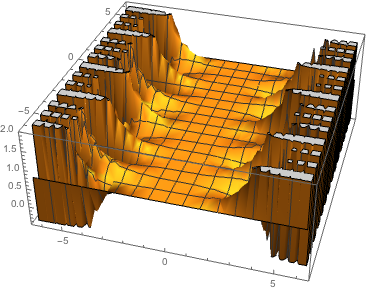
\includegraphics[scale=0.3]{lap_01_3} & 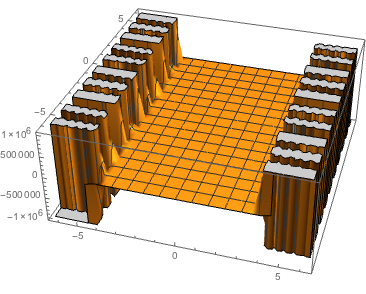
\includegraphics[scale=0.3]{lap_01_30} & 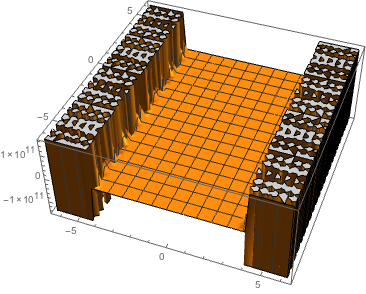
\includegraphics[scale=0.3]{lap_01_50}\\
\textit{The first 3 terms} & \textit{The first 30 terms} & \textit{The first 50 terms}
\end{tabular}
\end{center}
Plugging this infinite sum into mathematica tells us that it does not converge; the values are heading towards $\infty$ as the sum grows. We will leave our answer as a series, and we are done.


\newpage
\subsection{Wrapping Up}
\indent Before we move onto the next topic, we will present some common patterns amongst the second order PDEs. Below, you will find each of the three equations in the classical trinity, and their corresponding solutions based on the boundary conditions.
\subsubsection{The Heat Equation}
\[
\begin{array}{c c}
\begin{cases}
u_{t} - ku_{xx} = 0\\
u(0,t) = u(L,t) = 0\\
u(x,0) = f(x)
\end{cases}
&
\begin{cases}
u_{t} - ku_{xx} = 0\\
u_{x}(0,t) = u_{x}(L,t) = 0\\
u(x,0) = g(x)
\end{cases}\\
&\\
u(x,t) = \sum_{n=1}^{\infty}b_{n}e^{-k\left(\frac{n\pi}{L}\right)^{2}t}\sin{\left(\frac{n\pi x}{L}\right)}
& u(x,t) = \frac{a_{0}}{2} + \sum_{n=1}^{\infty}a_{n}e^{-k\left(\frac{n\pi}{L}\right)^{2}t}\cos{\left(\frac{n\pi x}{L}\right)}\\
&\\
\begin{cases}
u_{t} - ku_{xx} = 0\\
u(0,t) = u_{x}(L,t) = 0\\
u(x,0) = h(x)
\end{cases}
&
\begin{cases}
u_{t} - ku_{xx} = 0\\
u_{x}(0,t) = u(L,t) = 0\\
u(x,0) = k(x)
\end{cases}\\
&\\
u(x,t) =  \sum_{n=1}^{\infty}a_{n}e^{-k\left(\left[n + \frac{1}{2}\right]\frac{\pi}{L}\right)^{2}t}\sin{\left(\left[n + \frac{1}{2}\right]\frac{\pi x}{L}\right)}
& u(x,t) =  \sum_{n=1}^{\infty}a_{n}e^{-k\left(\left[n + \frac{1}{2}\right]\frac{\pi}{L}\right)^{2}t}\cos{\left(\left[n + \frac{1}{2}\right]\frac{\pi x}{L}\right)}
\end{array}
\]
\noindent\\
\subsubsection{The Wave Equation}
\[
\begin{array}{c c}
\begin{cases}
u_{tt} - c^{2}u_{xx} = 0\\
u(0,t) = u(L,t) = 0\\
u(x,0) = f(x) \quad u_{t}(x,0) = g(x)
\end{cases}
&
\begin{cases}
u_{tt} - c^{2}u_{xx} = 0\\
u_{x}(0,t) = u_{x}(L,t) = 0\\
u(x,0) = f(x) \quad u_{t}(x,0) = g(x)
\end{cases}\\
&\\
u(x,t) = \sum_{n=1}^{\infty}\left[a_{n}\cos{\left(\frac{n \pi t c}{L}\right)} + b_{n}\sin{\left(\frac{n \pi t c}{L}\right)}\right]\sin{\left(\frac{n \pi x}{L}\right)}
&u(x,t) = \frac{a_{0}}{2} + \sum_{n=1}^{\infty}\left[a_{n}\cos{\left(\frac{n \pi t c}{L}\right)} + b_{n}\sin{\left(\frac{n \pi t c}{L}\right)}\right]\cos{\left(\frac{n \pi x}{L}\right)}\\
&\\
\end{array}
\]
\[
\begin{array}{c}
\begin{cases}
u_{tt} - c^{2}u_{xx} = 0\\
u(0,t) = u_{x}(L,t) = 0\\
u(x,0) = f(x) \quad u_{t}(x,0) = g(x)
\end{cases}\\
\\
u(x,t) = a_{0} + b_{0}t + \sum_{n=1}^{\infty}\left[ a_{n}\cos{\left(\left[n + \frac{1}{2}\right]\frac{\pi t}{L}\right)} + b_{n}\sin{\left(\left[n + \frac{1}{2}\right]\frac{\pi x}{L}\right)}\right]\sin{\left(\left[n + \frac{1}{2}\right]\frac{\pi x}{L}\right)}\\
\\
\begin{cases}
u_{tt} - c^{2}u_{xx} = 0\\
u_{x}(0,t) = u(L,t) = 0\\
u(x,0) = f(x) \quad u_{t}(x,0) = g(x)
\end{cases}\\
\\
u (x,t) = a_{0} + b_{0}t + \sum_{n=1}^{\infty}\left[ a_{n}\cos{\left(\left[n + \frac{1}{2}\right]\frac{\pi t}{L}\right)} + b_{n}\sin{\left(\left[n + \frac{1}{2}\right]\frac{\pi x}{L}\right)}\right]\cos{\left(\left[n + \frac{1}{2}\right]\frac{\pi x}{L}\right)}
\end{array}
\]
\subsubsection{The Laplace Equation}
\paragraph{Cartesian Coordinates}
\[
\begin{array}{c c}
\begin{cases}
u_{xx} + u_{yy} = 0\\
u(0,y) = u(L,y) = 0
\end{cases}
&
\begin{cases}
u_{xx} + u_{yy} = 0\\
u_{x}(0,y) = u_{x}(L,y) = 0
\end{cases}\\
&\\
u(x,y) = \sum_{n=1}^{\infty}\left[a_{n}\sinh{\left(\frac{n \pi y}{L}\right)} + b_{n}\cosh{\left(\frac{n\pi y}{L}\right)}\right]\sin{\left(\frac{n\pi x}{L}\right)}
& u(x,y) = \sum_{n=1}^{\infty}\left[a_{n}\sinh{\left(\frac{n \pi y}{L}\right)} + b_{n}\cosh{\left(\frac{n\pi y}{L}\right)}\right]\cos{\left(\frac{n\pi x}{L}\right)}
\end{array}
\]
\\
\[
\begin{array}{c}
\begin{cases}
u_{xx} + u_{yy} = 0\\
u_{x}(0,y) = u(L,y) = 0
\end{cases}\\
\\
u(x,t) = \sum_{n=1}^{\infty}\left[a_{n}\sinh{\left(\left[n + \frac{1}{2}\right]\frac{\pi y}{L}\right)} + b_{n}\cosh{\left(\left[n + \frac{1}{2}\right]\frac{\pi y}{L}\right)}\right]\cos{\left(\left[n + \frac{1}{2}\right]\frac{\pi y}{L}\right)}\\
\\
\begin{cases}
u_{xx} + u_{yy} = 0\\
u(0,y) = u_{x}(L,y) = 0
\end{cases}\\
\\
u(x,t) = \sum_{n=1}^{\infty}\left[a_{n}\sinh{\left(\left[n + \frac{1}{2}\right]\frac{\pi y}{L}\right)} + b_{n}\cosh{\left(\left[n + \frac{1}{2}\right]\frac{\pi y}{L}\right)}\right]\sin{\left(\left[n + \frac{1}{2}\right]\frac{\pi y}{L}\right)}
\end{array}
\]
\paragraph{Polar Coordinates}
\begin{gather*}
\begin{cases}
u_{rr} + \frac{1}{r}u_{r} + \frac{1}{r^{2}}u_{\theta\theta} = 0\\
u(h,\theta) = f(\theta)\quad \text{on}\ x < \theta < L
\end{cases}\\
u(r,\theta) = a_{0} + \sum_{n=1}^{\infty}a_{n}r^{n}\cos{\left(\frac{n \pi \theta}{L}\right)} + b_{n}r^{n}\sin{\left(\frac{n \pi \theta}{L}\right)}
\end{gather*}
\newpage


\section{The Cauchy Problem}
\hrule
\noindent \\\\
\indent Up until now, we have always been given our PDE's with boundary conditions and initial values; but imagine that we did not have a boundary? The traditional method that we have been using would fail at this point. Since we would not be able to find any eigenvalues, we would not be able to form a series solution by using the \textit{Separation of Variables} technique. Let's consider the familiar heat equation:
\[
\begin{cases}
\xi_{t} - k\xi_{xx} = 0\\
\xi(x,0) = f(x)
\end{cases}
\]
Through much careful derivation and theory, we can say that the general solution for this problem will be
\[
\xi(x,t) = \frac{1}{\sqrt{4 \pi k t}}\int_{-\infty}^{\infty}e^{-\frac{(x-y)^{2}}{4kt}}f(y)dy.
\]
The question now should be ``How can we solve this?'' The first step we will take is letting
\[
u = \frac{y-x}{\sqrt{4kt}}.
\]
We are going to perform a \textit{u substitution} to try and put this integral into a nicer form. This yields
\begin{align*}
y &= x + u\sqrt{4kt}\\
dy &= \sqrt{4kt}\ du.
\end{align*}
This changes our original problem into
\[
\xi(x,t) = \frac{1}{\sqrt{\pi}}\int_{-\infty}^{\infty}e^{-u^{2}}f(x+u\sqrt{4kt})du.
\]
Let's look at an example\\\\
\noindent \textbf{\textit{Ex:}} Solve the following PDE
\[
\begin{cases}
\mu_{t} - k\mu_{xx} = 0\\
\mu(x,0) = \cos{x}
\end{cases}
\]
\indent \textbf{\textit{Solution:}} From above, we know what our general solution will look like. All we need to do is substitute in our initial condition. We have the following:
\begin{align*}
\mu(x,t) &= \frac{1}{\sqrt{\pi}}\int_{-\infty}^{\infty}e^{-u^{2}}\cos{(x + u\sqrt{4kt})}du\\
&= \frac{1}{\sqrt{\pi}}\int_{-\infty}^{\infty}e^{-u^{2}}\left[\cos{(x)}\cos{(u\sqrt{4kt})} - \sin{(x)}\sin{(u\sqrt{4kt})}\right]du\\
&=  \frac{2}{\sqrt{\pi}}\cos{(x)}\int_{0}^{\infty}e^{-u^{2}}\cos{(u\sqrt{4kt})}du.
\end{align*}
You may be wondering what happened to the $\sin$ terms. Recall that $\sin$ is an odd function, so it will ultimately be $0$ on the interval $[-\infty,\infty]$; because of this fact, we can remove it now. We also use the face that the $\cos$ is even, so it is okay to halve the interval and multiply by two. Now we need to evaluate this integral. We will substitute $\alpha = \sqrt{4kt}$, and assign a function, $\Upsilon(\alpha)$, to the integral. This gives us the following system:
\[
\begin{cases}
\Upsilon(\alpha) = \int_{0}^{\infty}e^{-u^{2}}\cos{(\alpha u)}du\\
\Upsilon(0) = \int_{0}^{\infty}e^{-u^{2}}du\\
\end{cases}
\]
Believe it or not, we actually know the answer to $\Upsilon(0)$. To find it, we can assign a function to the integral in a similar fashion as we have already done. Calling it $\Psi$, we have
\begin{align*}
\Psi &= \int_{0}^{\infty}e^{-u^{2}}du\\
\Psi^{2} &= \int_{0}^{\infty}e^{-u^{2}}du \int_{0}^{\infty}e^{-v^{2}}dv\\
\Psi^{2} &= \int_{0}^{\infty}\int_{0}^{\infty}e^{-u^{2}-v^{2}}dudv\\
\Psi^{2} &= \int_{0}^{\pi/2}\int_{0}^{\infty}re^{-r^{2}}drd\theta\\
\Psi^{2} &= \frac{\pi}{2}\left[-\frac{1}{2}e^{-r^{2}}\right]\Bigg |_{r=0}^{r=\infty}\\
\Psi^{2} &= \frac{\pi}{4}\\
\Psi &= \frac{\sqrt{\pi}}{2}.
\end{align*}
So we know that $\Upsilon(0) = \frac{\sqrt{\pi}}{2}$. Plugging this into our system gives us
\[
\begin{cases}
\Upsilon(\alpha) = \int_{0}^{\infty}e^{-u^{2}}\cos{(\alpha u)}du\\
\Upsilon(0) = \frac{\sqrt{\pi}}{2}\\
\end{cases}
\]
Now, we will take the derivative of $\Upsilon$. This gives us
\[
\Upsilon'(\alpha) = -\int_{0}^{\infty}ue^{-u^{2}}\sin{(\alpha u)}du.
\]
Integration by parts gives us
\[
\frac{1}{2}e^{-u^{2}}\sin{(\alpha u)}\Big |_{0}^{\infty} - \alpha\int_{0}^{\infty}\frac{1}{2}e^{-u^{2}}\cos{(\alpha u)}du.
\]
The value from $0$ to $\infty$ is zero, since the $\sin$ function odd. This leaves us with following relationship:
\[
\Upsilon'(\alpha) = -\frac{\alpha}{2}\Upsilon(\alpha) \alpha.
\]
We can solve this as an ODE. It's separable, so we get
\begin{align*}
\frac{d\Upsilon}{\Upsilon} &= -\frac{\alpha}{2}d\alpha\\
\ln{(\Upsilon)} &= -\frac{\alpha^{2}}{4} + c_{1}\\
\Upsilon &= c_{2}e^{-\frac{\alpha^{2}}{4}}.
\end{align*}
Applying the initial condition gives us
\[
\Upsilon = \frac{\sqrt{\pi}}{2}e^{-\frac{\alpha^{2}}{4}}.
\]
Substituting back in gives us a final answer of
\begin{align*}
\mu(x,t) &= \frac{2}{\sqrt{\pi}}\cos{x}\Upsilon(\sqrt{4kt})\\
&= \cos{x}e^{-kt},
\end{align*}
and we are done.


\newpage
\indent Now we will move on to the Cauchy wave equation. We will be presented with a similar problem: a wave equation on an unbounded domain. Consider the following problem:
\noindent \\\\
\noindent \textbf{\textit{Ex:}} Solve the following PDE
\[
\begin{cases}
u_{tt} - c^{2}u_{xx} = 0\\
u(x,0) = \sin{x}\\
u_{t}(x,0) = \cos{x}
\end{cases}
\]
\indent \textbf{\textit{Solution:}} Just as with the heat equation, we have a formal solution for the homogeneous wave equation. We will do the derivation, but I will tell you that the formal solution is
\[
u(x,t) = \frac{1}{2}\left[f(x+ct) + f(x-ct)\right] + \frac{1}{2c}\int_{x-ct}^{x+ct}g(s)\mathop{ds}.
\]
Now let's derive the formal solution. We want a solution in the form of
\[
u(x,t) = F(x+ct) + G(x-ct).
\]
Now we can say that $u_{t} = cF'(x+ct) - cG'(x-ct)$, and $u_{t}(x,0) = cF'(x) - cG'(x)$. This means
\begin{align*}
F(x) + G(x) &= f(x)\\
F(x) - G(x) &= \frac{1}{c}\int_{0}^{x}g(s)\mathop{ds} + c_{1}.
\end{align*}
Solving the system yields
\begin{align*}
u(x,t) &= \frac{1}{2} f(x+ct) + \frac{1}{2c}\int_{0}^{x+ct}g(s)\mathop{ds} + \frac{c_{1}}{2} + \frac{1}{2}f(x-ct) -\frac{1}{2c}\int_{0}^{x-ct}g(s)\mathop{ds} - \frac{c_{1}}{2}\\
&= \frac{1}{2}\left[f(x+ct) + f(x-ct)\right] + \frac{1}{2c}\int_{x-ct}^{x+ct}g(s)\mathop{ds},
\end{align*}
and that is the derivation. This problem is simply plugging into the formal solution. We have the following:
\begin{align*}
u(x,t) &= \frac{1}{2}\left[\sin{(x+ct)} + \sin{(x-ct)}\right] + \frac{1}{2c}\int_{x-ct}^{x+ct}\cos{(s)}\mathop{ds}\\
&= \frac{\sin{(x+ct)} + \sin{(x-ct)}}{2} + \frac{\cos{(x)}\sin{(ct)}}{c}\\
&=  \frac{\cos{(x)}\sin{(ct)}}{c} + \cos{(ct)}\sin{(x)},
\end{align*}
and we are done.


\newpage
\indent So far, we have only dealt with homogeneous Cauchy problems. We will now look at the case where we have a non-homogeneous problem. The first variation of this problem is the \textit{half-line} problem. In this problem, we will have a bound on our equation, and we will generalize the solution so that we are dealing with an unbounded Cauchy problem. Let's look at an example.
\noindent\\\\ \textbf{\textit{Ex:}} Solve the following PDE
\[
\begin{cases}
u_{t} - ku_{xx} = 0\\
u(x,0) = \phi(x)\\
u(0,t) = 0
\end{cases}
\]
\indent \textbf{\textit{Solution:}} We have both an initial condition and a boundary condition here. This problem is saying that at $x=0$, there is an impassable boundary. This forces our domain to be $[0,\infty)$. To solve a Cauchy problem, however, we want a domain of $(-\infty,\infty)$. We can force this domain by extending our initial condition, $\phi(x)$, over the boundary. We have the following rule:
\[
\phi_{0}(x) =
\begin{cases}
\phi(x)\quad\quad x>0\\
-\phi(-x)\ x<0.
\end{cases}
\]
Now we are dealing with the system
\[
\begin{cases}
u_{t} - ku_{xx} = 0\\
u(x,0) = \phi_{0}(x),
\end{cases}
\]
which we can solve using the formal solution to the heat equation. Recall that
\[
u(x,t) = \frac{1}{\sqrt{4k\pi t}}\int_{-\infty}^{\infty}e^{-\frac{(x-y)^{2}}{4kt}}\phi_{0}(y)\mathop{dy}.
\]
Substituting into the equation gives us
\begin{align*}
u(x,t) &= \frac{1}{\sqrt{4k\pi t}}\left[\int_{0}^{\infty}e^{-\frac{(x-y)^{2}}{4kt}}\phi(y)\mathop{dy} + \int_{-\infty}^{0}e^{-\frac{(x-y)^{2}}{4kt}}(-\phi(-y))\mathop{dy} \right]\\
&= \frac{1}{\sqrt{4k\pi t}}
\end{align*}
\end{document}
